\ChapterImageStar[cap:validacion]{Implementación y validación de la solución}{./images/fondo.png}\label{cap:validacion}
\mbox{}\\
La presente sección tiene como finalidad validar la efectividad de la arquitectura de defensa en profundidad implementada mediante la 
integración de OPNsense, Suricata y Wazuh dentro de un laboratorio virtualizado. Para ello, se diseñaron ocho casos de prueba basados en el 
marco MITRE ATT\&CK y las fases de la Cyber Kill Chain, permitiendo evaluar capacidades de detección, correlación de eventos y respuesta 
activa frente a diferentes escenarios de ataque.

Las pruebas fueron ejecutadas desde una máquina atacante con OpenSUSE, generando tráfico y eventos maliciosos controlados dentro de un 
entorno completamente aislado. De esta manera, fue posible analizar el comportamiento de la arquitectura propuesta y validar la capacidad 
de monitoreo continuo, mitigación dinámica y gestión centralizada de eventos de seguridad.

\section{Metodología de ejecución de pruebas}
\noindent

Con el fin de validar los aspectos de seguridad integrados mediante la arquitectura de defensa en profundidad implementada, se definió una 
metodología orientada a garantizar la reproducibilidad y validez de los resultados obtenidos en los ocho escenarios de prueba planteados. 
Para ello, cada caso fue ejecutado bajo un protocolo estandarizado compuesto por cuatro fases consecutivas:

\begin{itemize}
    \item \textbf{Fase de Línea Base:} verificación previa del estado operativo de la infraestructura, comprobando el funcionamiento de los agentes de Wazuh, el motor Suricata y la conectividad entre las máquinas involucradas.
    
    \item \textbf{Fase de Estímulo:} ejecución controlada del ataque o actividad maliciosa desde la máquina atacante mediante las herramientas definidas para cada escenario.
    
    \item \textbf{Fase de Monitoreo y Centralización:} observación del procesamiento de eventos y generación de alertas por parte de Wazuh, así como el tiempo de reacción de la respuesta activa.
    
    \item \textbf{Fase de Verificación de Contención:} comprobación de la mitigación aplicada mediante las reglas dinámicas del firewall y la interrupción de la actividad maliciosa.
\end{itemize}

\subsection{Criterios de validación}
\noindent

Con el fin de evaluar cuantitativa y cualitativamente el desempeño de la arquitectura de defensa en profundidad, se definieron criterios 
estrictos para dictaminar el estado final de cada prueba:

\subsubsection{Criterio de Éxito (Aprobado)}
\noindent

Una prueba se considera exitosa si cumple de manera secuencial el ciclo completo de automatización definido en la arquitectura 
implementada: detección del tráfico malicioso por parte del host o del IDS Suricata, reporte del evento hacia el Wazuh Manager, correlación 
de la regla y generación de la alerta correspondiente en el Dashboard, y finalmente la aplicación de la respuesta activa mediante el 
firewall OPNsense, bloqueando la dirección IP atacante en un tiempo igual o inferior al umbral crítico de tolerancia establecido.

No obstante, es importante resaltar que no todas las alertas generadas producen una respuesta activa automática. Wazuh evalúa el nivel de s
everidad asociado a cada evento y únicamente ejecuta acciones de mitigación cuando la alerta supera el umbral de prioridad configurado. 
Por consiguiente, aquellos eventos catalogados con niveles inferiores a 10 dentro de la escala de criticidad del SIEM son considerados de 
bajo impacto y no desencadenan interacción directa con el firewall.

\subsubsection{Criterio de Fallo (Rechazado)}
\noindent

Una prueba se considera fallida cuando se presenta alguna anomalía que interrumpa el ciclo de detección, correlación o contención definido 
en la arquitectura de seguridad implementada. Entre los posibles escenarios de fallo se encuentran la evasión del ataque frente a las 
firmas del IDS o los registros del sistema, generando falsos negativos; la incapacidad del agente para transmitir la alerta debido a 
congestión o fallos en el canal seguro de comunicación; errores en el procesamiento de las reglas de respuesta activa por parte del Wazuh 
Manager; o la imposibilidad del firewall OpnSense de aplicar el bloqueo perimetral correspondiente. Cualquiera de estas situaciones 
implica que el atacante conserve conectividad y logre continuar o completar la explotación del objetivo.

\section{Desarrollo de los casos de prueba}
\noindent

El propósito de este apartado es consolidar y describir los ocho (8) casos de prueba ejecutados sobre el entorno virtualizado en el que se 
implementó la arquitectura de defensa en profundidad. En cada escenario se especifica el origen del ataque, la técnica empleada y el 
comportamiento de los componentes de seguridad desplegados, evaluando la capacidad de detección del IDPS Suricata, la correlación de 
eventos realizada por el SIEM Wazuh y la aplicación de medidas de contención mediante la respuesta activa integrada con el firewall 
OpnSense.

Lo anterior permite determinar la efectividad de los aspectos de seguridad implementados y su alineación con los lineamientos establecidos 
en las normas \ISO/IEC 27001:2022 e \ISO/IEC 27017:2015, verificando la capacidad de la infraestructura para proteger los activos y 
servicios del grupo GRID frente a diferentes escenarios de amenaza. A continuación, se presenta la descripción de cada una de las 
pruebas realizadas.

\subsection{Configuración del entorno de red para la ejecución de casos de prueba}
\noindent

Para el desarrollo de los casos de prueba descritos a continuación, se implementaron dos reglas DNAT (Destination Network Address 
Translation) en el firewall OpnSense, con el propósito de exponer de forma controlada los servicios SSH y HTTP de la red interna hacia la 
red WAN simulada. En ambas reglas se definió el protocolo TCP, debido a que dichos servicios operan exclusivamente sobre este protocolo, 
siguiendo el principio de mínimo privilegio.

Esta configuración permitió redirigir el tráfico entrante dirigido a la interfaz WAN hacia la máquina objetivo ubicada en la red de 
servidores internos, replicando un escenario real de exposición de servicios hacia redes externas no confiables. De esta manera, fue 
posible ejecutar ataques controlados sobre la máquina objetivo y evaluar la capacidad de detección, correlación y mitigación de amenazas 
por parte de la arquitectura de seguridad implementada. En la figura~\ref{fig1} se demuestra la creación y parámetros de la virtual IP y en 
la figura~\ref{fig2} se evidencia la configuración de las reglas DNAT establecidas.


\begin{figure}[H]
	\centering
	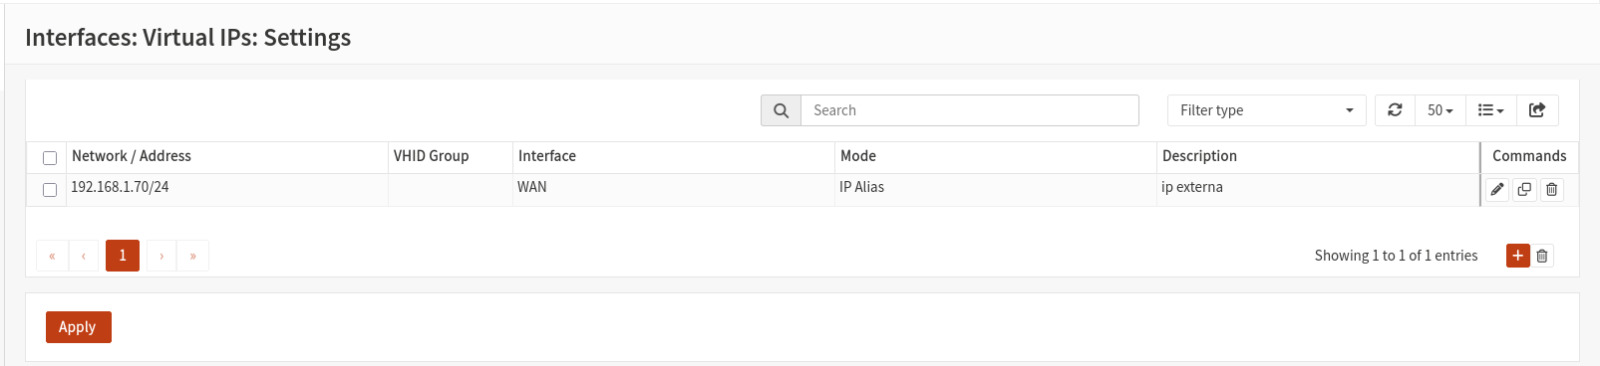
\includegraphics[scale=0.2]{tablas-images/pruebas/vali-1.jpeg}
	\caption{Configuración de virtual IP}\label{fig1}
\end{figure}


\begin{figure}[H]
	\centering
	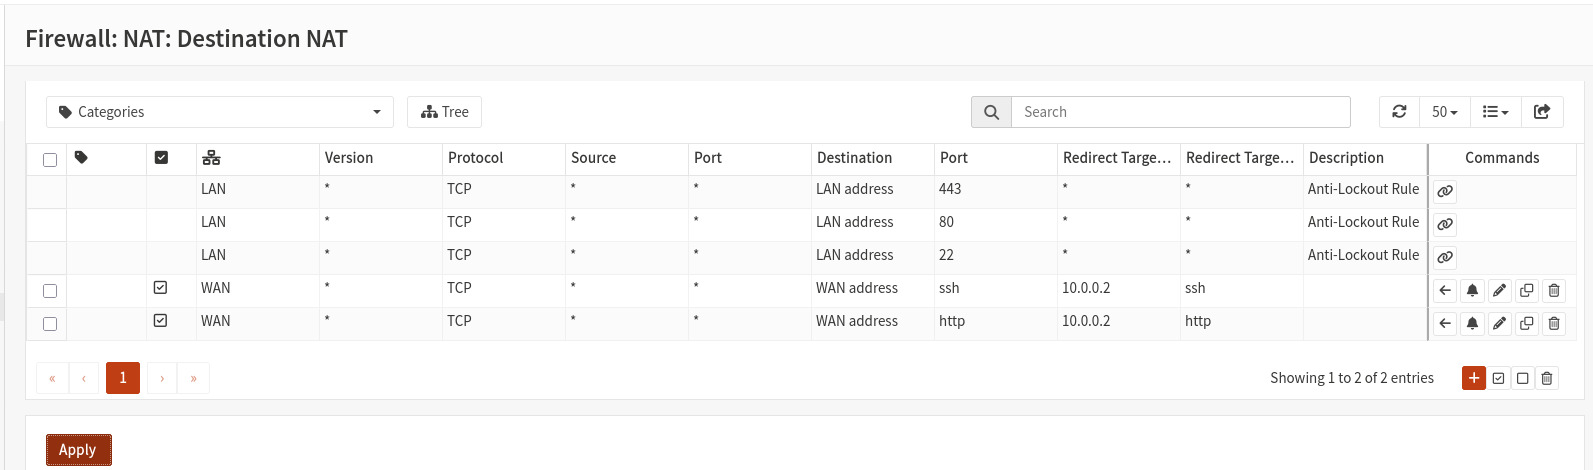
\includegraphics[scale=0.2]{tablas-images/pruebas/vali-2.jpeg}
	\caption{Configuración de las reglas DNAT}\label{fig2}
\end{figure}

Adicionalmente, fue necesario deshabilitar las opciones de bloqueo de redes privadas y redes Bogon en la interfaz WAN de OpnSense, debido a 
que el entorno virtualizado del laboratorio emplea direccionamiento IP privado en los segmentos de red utilizados. Esta configuración 
permitió habilitar el tránsito del tráfico entre la red atacante y la máquina objetivo, garantizando la correcta ejecución de los escenarios 
de prueba. En la figura~\ref{fig3} se evidencia la deshabilitación de las opciones \textit{Block private networks} y \textit{Block bogon 
networks}.

\begin{figure}[H]
	\centering
	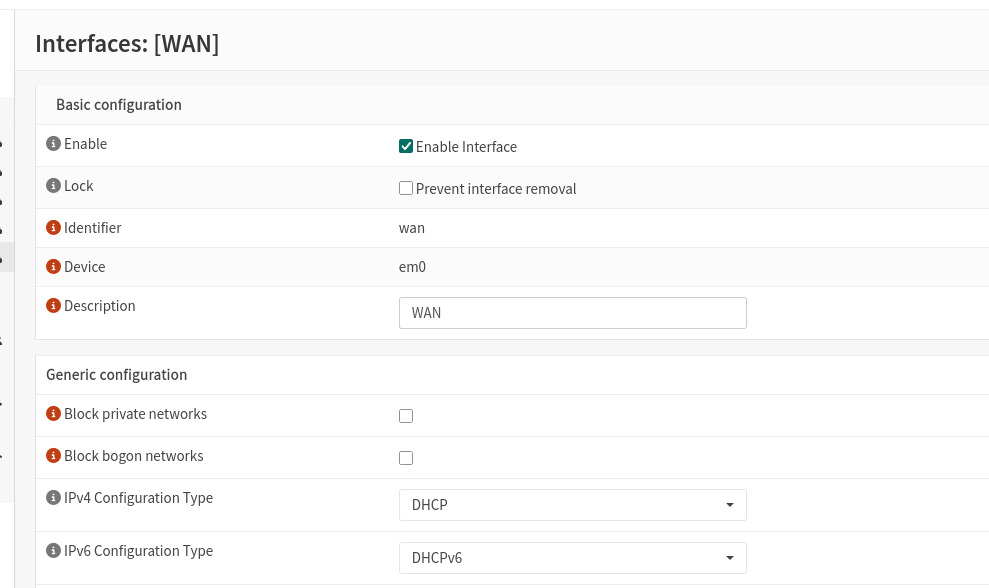
\includegraphics[scale=0.2]{tablas-images/pruebas/vali-3.jpeg}
	\caption{Deshabilitación de opciones de bloqueo de tráfico de red}\label{fig3}
\end{figure}

Asimismo, durante la configuración de las reglas DNAT previamente definidas, se habilitó la opción de creación automática de reglas de 
firewall asociadas a cada traducción realizada sobre la interfaz WAN. Esto permitió autorizar de manera automática el tránsito del 
tráfico de red hacia los servicios expuestos, evitando la necesidad de crear reglas manuales adicionales. La figura~\ref{fig4} presenta el 
contexto visual de la configuración aplicada.

\begin{figure}[H]
	\centering
	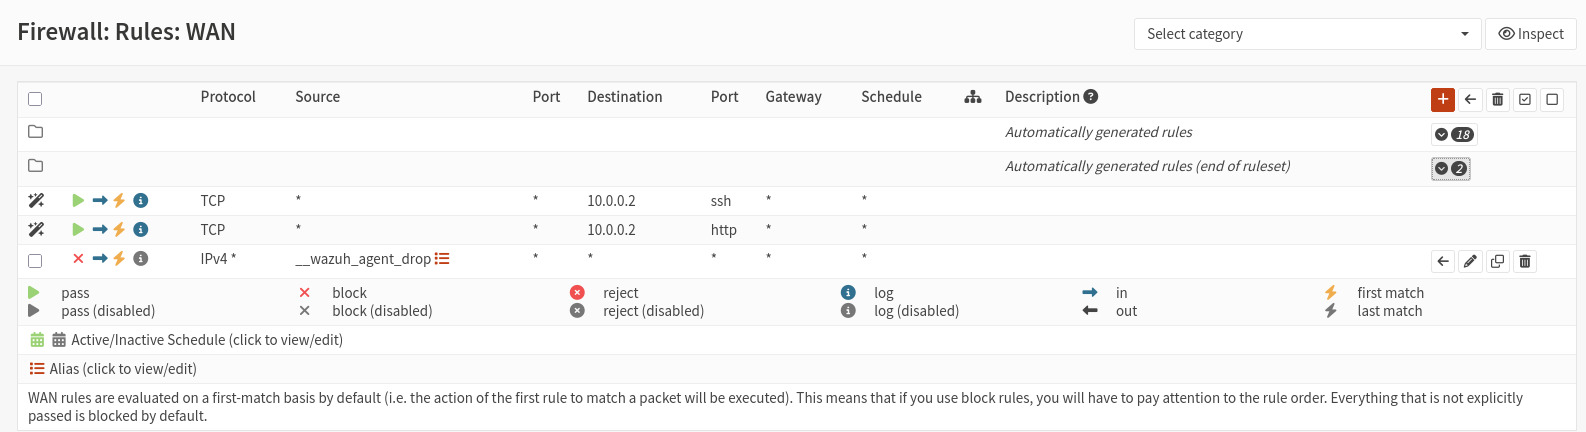
\includegraphics[scale=0.2]{tablas-images/pruebas/vali-4.jpeg}
	\caption{Reglas creadas automáticamente a partir de las DNAT}\label{fig4}
\end{figure}

De igual forma, en la Figura~\ref{fig5} se evidencia la adecuación de las reglas necesarias para permitir el tránsito desde la interfaz 
SERVERS hacia los servicios SSH y HTTP mediante la dirección IP virtual especificada anteriormente. Esta configuración tuvo como finalidad 
habilitar la ejecución de las pruebas y simular de manera adecuada la exposición controlada de servicios por parte de la máquina objetivo.

\begin{figure}[H]
	\centering
	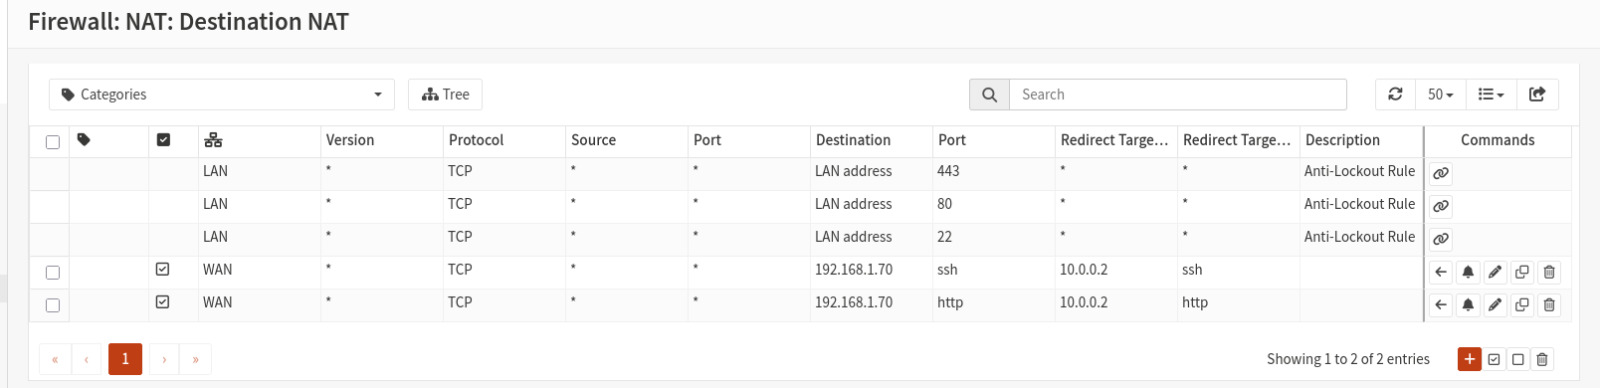
\includegraphics[scale=0.2]{tablas-images/pruebas/vali-5.jpeg}
	\caption{Reglas creadas automáticamente para la interfaz SERVERS}\label{fig5}
\end{figure}

\subsection{Caso de Prueba 1 (CP-01) Escaneo de Puertos Mediante Nmap}
\noindent

Para la primera prueba, se establece que la fase de reconocimiento constituye la etapa inicial de cualquier ataque informático, en la cual 
el adversario identifica servicios expuestos y posibles vectores de explotación sobre la infraestructura objetivo. En este caso de prueba, 
se simuló un actor externo ejecutando un escaneo de red desde la WAN hacia la dirección IP virtual del firewall OPNsense, con el propósito 
de validar la capacidad del sistema de detección y respuesta para identificar, alertar y mitigar de forma automatizada este tipo de 
actividad maliciosa.

\subsubsection{Objetivo de la prueba}
\noindent

Verificar que el sistema de defensa en profundidad implementado, compuesto por las herramientas de código abierto Wazuh, Suricata y 
OPNsense, detecte un escaneo de reconocimiento proveniente desde la red WAN, genere alertas asociadas a la firma identificada y ejecute la 
respuesta activa mediante el bloqueo perimetral automatizado una vez superado el umbral de tolerancia establecido. Dicho umbral se activa 
cuando se registran más de cinco alertas del mismo tipo en un intervalo de 60 segundos.

\subsubsection{Herramienta Utilizada}
\noindent

La herramienta utilizada fue Nmap (Network Mapper), una utilidad de código abierto ampliamente empleada en el ámbito de la seguridad 
informática para el descubrimiento de redes y la auditoría de seguridad. Esta permite identificar hosts activos, puertos abiertos, 
servicios en ejecución y sus respectivas versiones mediante el envío de paquetes construidos de manera específica.

Para este caso de prueba se utilizó el siguiente comando:

\begin{lstlisting}[language=bash, caption={Comando Nmap utilizado para el escaneo de reconocimiento}, label={lst:nmap_scan}]

sudo nmap -sS -Pn -sV -p 22,80 192.168.170

\end{lstlisting}

En donde cada parámetro cumple una función específica, tal como se describe en la Tabla~\ref{tab:parametros_nmap}.

\begin{table}[H]
\centering
\caption{Descripción de Parámetros para NMAP}\label{tab:parametros_nmap}
\begin{tabular}{|c|p{9cm}|}
\hline
\textbf{Parámetro} & \textbf{Descripción} \\ \hline

\texttt{-sS} & Realiza un escaneo SYN sigiloso, no completa el \textit{handshake} TCP, pero envía paquetes SYN a cada puerto. \\ \hline

\texttt{-Pn} & Omite la detección de host activo mediante \textit{ping}. \\ \hline

\texttt{-sV} & Detecta la versión de los servicios en los puertos encontrados mediante el envío de grandes volúmenes de paquetes luego de detectar un puerto abierto. \\ \hline

\texttt{-p 22,80} & Limita el escaneo a los puertos correspondientes a SSH y HTTP. \\ \hline

\end{tabular}
\end{table}

\subsubsection{Ejecución de la prueba}
\noindent

Este apartado se desarrolló desde la máquina atacante OpenSUSE, desde la cual se ejecutó un escaneo de reconocimiento sobre la dirección 
IP virtual configurada en OPNsense \texttt{192.168.1.70}, expuesta a través de la interfaz WAN del firewall. Para ello, se utilizó el 
comando descrito en el apartado anterior, replicando el comportamiento de un atacante real en un entorno donde el objetivo puede 
encontrarse protegido mediante reglas ICMP.

El escaneo inicial, evidenciado en la figura~\ref{fig6}, permitió identificar los servicios activos sobre los puertos 22 y 80, obteniendo 
información relacionada con las versiones del software en ejecución y el sistema operativo del objetivo. Asimismo, fue necesario utilizar 
el comando \texttt{date} para verificar el tiempo exacto en el que inició la ejecución del comando Nmap.

\begin{figure}[H]
	\centering
	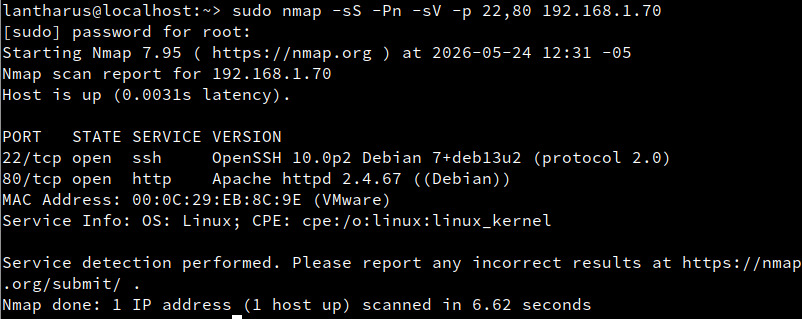
\includegraphics[scale=0.2]{tablas-images/pruebas/vali-6.jpeg}
	\caption{Escaneo Inicial a la máquina objetivo}\label{fig6}
\end{figure}

Una vez ejecutado el comando Nmap, el resultado esperado corresponde al bloqueo de la dirección IP desde la cual se realizó el escaneo. 
Esto puede verificarse al intentar reiterar el mismo procedimiento posteriormente. En el siguiente apartado se evaluará el comportamiento 
interno de la arquitectura de defensa en profundidad y se verificará si cumple con los criterios establecidos previamente.

\subsubsection{Resultados y Evidencias}
\noindent

El escaneo inicial permitió al atacante identificar los servicios expuestos en la dirección IP virtual, obteniendo información sensible de 
la máquina objetivo. No obstante, el tráfico generado fue interceptado por Suricata, el cual produjo múltiples alertas de reconocimiento, 
entre las que se destaca la firma \textit{“ET SCAN Nmap Scripting Engine User Agent Detected”}, categorizada como \textit{Web Application 
Attack} y con un nivel de confianza \textit{High}. En la Figura~\ref{fig7} se evidencia el flujo de registros capturados por Suricata en el archivo 
\texttt{eve.json}.

\begin{figure}[H]
	\centering
	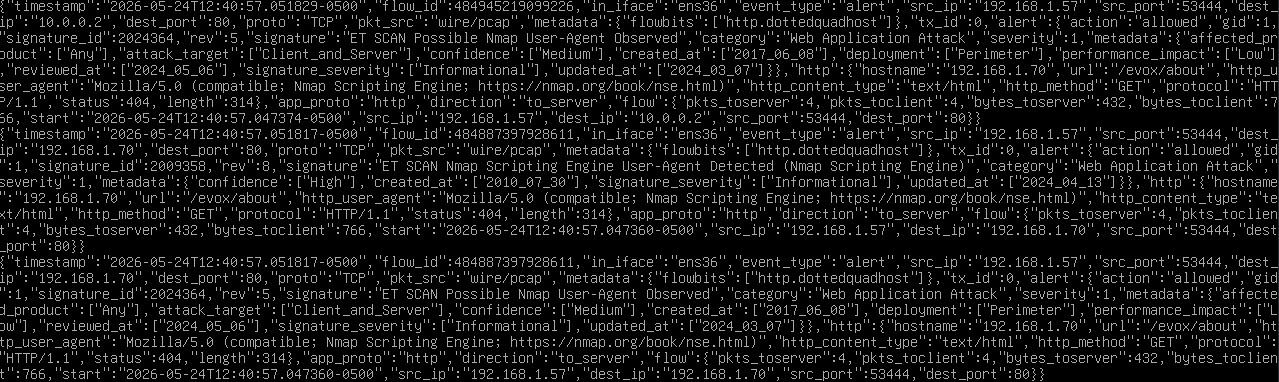
\includegraphics[scale=0.2]{tablas-images/pruebas/vali-7.jpeg}
	\caption{Escaneo Inicial a la máquina objetivo}\label{fig7}
\end{figure}

Una vez superado el umbral de tolerancia establecido, es decir, al generarse más de cinco alertas de reconocimiento por parte de Suricata, 
el Wazuh Manager correlacionó los eventos y activó la respuesta activa a las 12:40:51, ordenando al agente de OpnSense inyectar la 
dirección IP atacante \texttt{192.168.1.57} en la tabla de bloqueo \texttt{\_\_wazuh\_agent\_drop} a las 12:40:58.

El escaneo fue ejecutado a las 12:40:50, logrando la contención del ataque en un tiempo aproximado de 8 segundos desde el inicio del 
escaneo, valor considerablemente inferior al umbral crítico de 30 segundos definido en la metodología. En la figura~\ref{fig8} se evidencia la 
primera alerta reconocida por Wazuh y en la figura~\ref{fig9} el registro correspondiente a la respuesta activa ejecutada por OpnSense.

\begin{figure}[H]
	\centering
	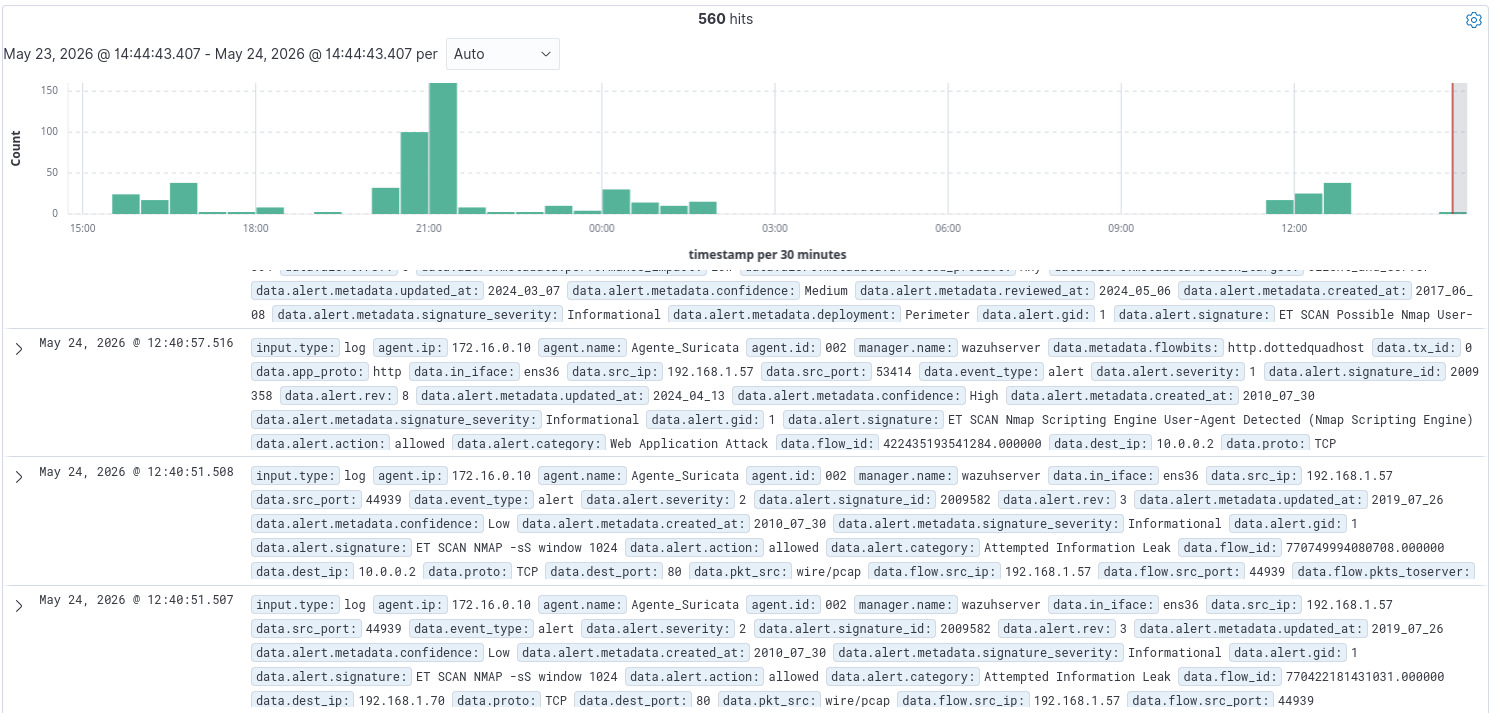
\includegraphics[scale=0.2]{tablas-images/pruebas/vali-8.jpeg}
	\caption{Dashboard de Wazuh emitiendo alertas}\label{fig8}
\end{figure}

\begin{figure}[H]
	\centering
	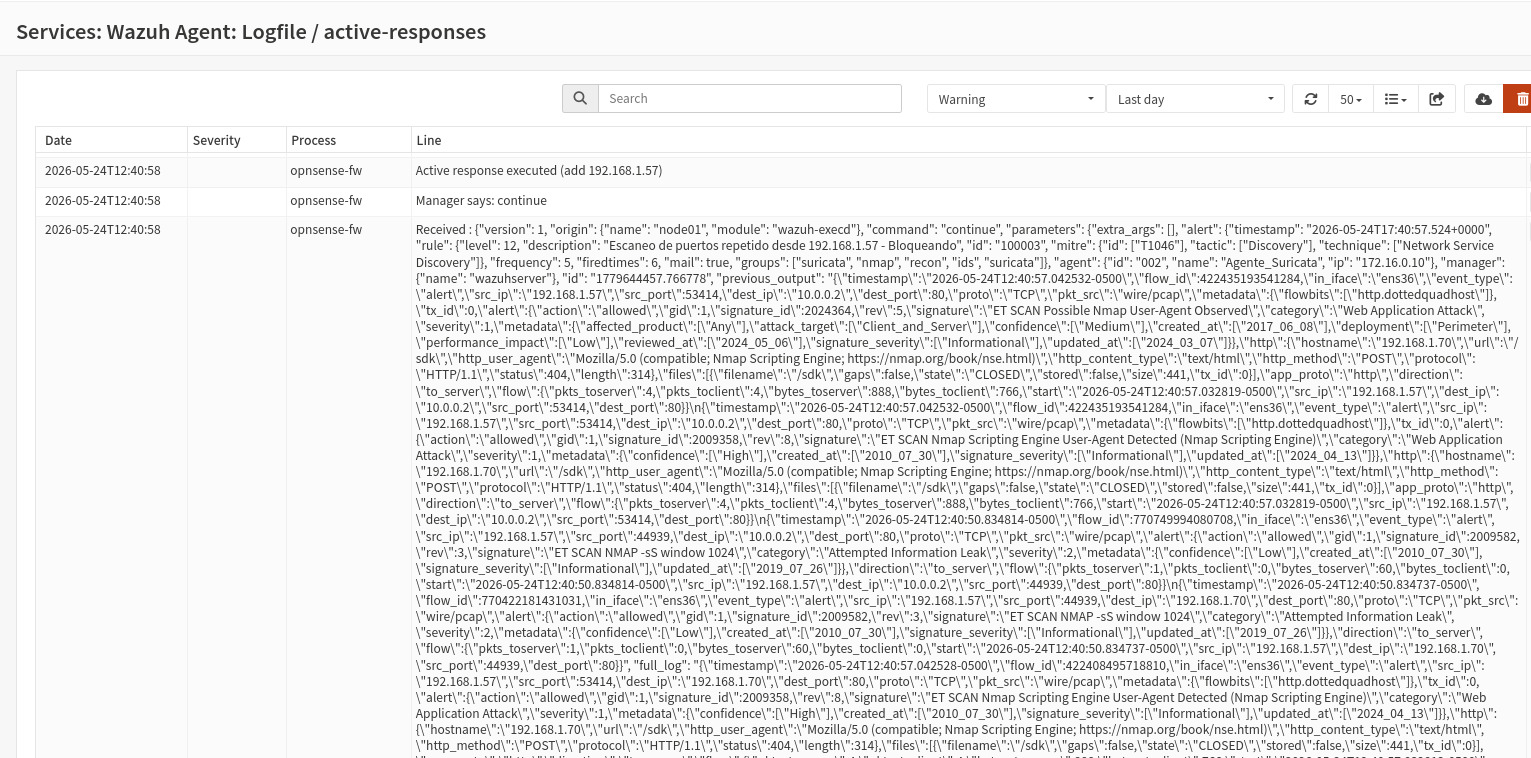
\includegraphics[scale=0.2]{tablas-images/pruebas/vali-9.jpeg}
	\caption{Registro de Instrucción de Respuesta Activa en OpnSense}\label{fig9}
\end{figure}

Tras la activación automática del mecanismo de respuesta activa por parte de Wazuh, se procedió a ejecutar un segundo escaneo utilizando 
los mismos parámetros, con el propósito de verificar la efectividad del bloqueo perimetral aplicado por OPNsense. Los resultados obtenidos 
se presentan en la figura~\ref{fig10}.

\begin{figure}[H]
	\centering
	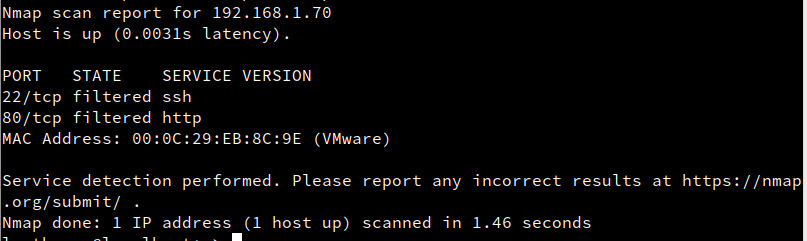
\includegraphics[scale=0.2]{tablas-images/pruebas/vali-10.jpeg}
	\caption{Ejecución de comando Nmap posterior a la respuesta activa}\label{fig10}
\end{figure}

El cambio de estado de \textit{“open”} a \textit{“filtered”} confirma que OPNsense descarta los paquetes provenientes del atacante debido 
al bloqueo aplicado mediante la respuesta activa. Adicionalmente, el tiempo de escaneo se redujo de 6.49 a 1.46 segundos, dado que Nmap no 
recibió respuesta alguna por parte del objetivo.

\subsubsection{Análisis del ciclo de detección}
\noindent

El caso de prueba permitió validar el funcionamiento integral del pipeline de detección y respuesta automatizada implementado en el 
laboratorio propuesto. El escaneo ejecutado desde la red WAN generó tráfico TCP SYN dirigido hacia los puertos 22 y 80 de la dirección IP 
virtual. Dicho tráfico fue capturado simultáneamente por Suricata a través de la interfaz en modo promiscuo conectada al \texttt{bridge0} 
de la red de OPNsense, garantizando visibilidad completa del tráfico y permitiendo la inspección profunda de paquetes en paralelo al 
procesamiento perimetral del firewall.

Las alertas generadas por Suricata fueron enviadas al Wazuh Manager mediante el agente instalado en la máquina del IDPS. Posteriormente, 
la regla personalizada \texttt{100003} correlacionó los eventos y elevó la alerta al nivel 12 una vez superado el umbral de cinco alertas 
consecutivas de reconocimiento, activando de forma automática el mecanismo de respuesta activa.

El ciclo completo de detección y contención se completó en 8 segundos desde la ejecución del escaneo, distribuyéndose aproximadamente en 
1.5 segundos para la detección y 6.5 segundos para la ejecución de la respuesta activa, cumpliendo satisfactoriamente el umbral crítico de 
30 segundos definido en la metodología.

El caso de prueba se clasifica como \textbf{Aprobado}, debido a que el ciclo completo de detección, correlación y bloqueo perimetral se 
ejecutó de manera secuencial y automatizada, impidiendo actividades posteriores de reconocimiento sobre el laboratorio virtual.

\subsection{Caso de prueba 2 (CP-02) Ataque de Fuerza Bruta Hydra}
\noindent

Los ataques de fuerza bruta representan una de las amenazas más frecuentes contra los servicios de acceso remoto, consistiendo en el 
intento sistemático de múltiples combinaciones de credenciales hasta obtener acceso no autorizado. El servicio SSH constituye uno de los 
objetivos más comunes debido a su amplio uso en la administración remota de sistemas.

Para este caso de prueba se simuló un ataque de fuerza bruta desde la red WAN hacia la dirección IP virtual expuesta, con el propósito de 
validar la capacidad del sistema de detección y respuesta para identificar y mitigar la amenaza de manera automatizada.

\subsubsection{Objetivo de la prueba}
\noindent

Verificar que el modelo de defensa en profundidad implementado detecte un ataque de fuerza bruta dirigido al servicio SSH, genere alertas 
de tráfico malicioso por parte de Suricata y envíe los eventos correspondientes al Wazuh Manager, activando posteriormente el mecanismo de 
respuesta activa para bloquear la dirección IP atacante antes de que se logre un acceso no autorizado a la máquina objetivo.

\subsubsection{Herramienta Utilizada}
\noindent

\subsubsection{Ejecución de la prueba}
\noindent

\subsubsection{Resultados y Evidencias}
\noindent

\subsubsection{Análisis del ciclo de detección}
\noindent

\subsection{Caso de prueba 2 (CP-02) Ataque de Fuerza Bruta Hydra}
\noindent

\subsubsection{Objetivo de la prueba}
\noindent

\subsubsection{Herramienta Utilizada}
\noindent

\subsubsection{Ejecución de la prueba}
\noindent

\subsubsection{Resultados y Evidencias}
\noindent

\subsubsection{Análisis del ciclo de detección}
\noindent

\section{Conclusiones de la validación}
\noindent

